\providecommand{\main}{../..}
\documentclass[\main/notes.tex]{subfiles}

\begin{document}
	\setcounter{chapter}{7}
	\chapter{Management Information and Decision Support Systems}
	\chaptermark{MIS and DSS}
		\section{Decision-Making and Problem-Solving}
			\begin{definition}{Decision-Making Phase}
				The first part of problem-solving, including three stages: intelligence, design, and choice.
			\end{definition}
			\begin{definition}{Problem-Solving}
				A process that goes beyond decision-making to include the implementation and monitoring stages.
			\end{definition}
			\begin{sidenote}{Decision-Making and Problem-Solving}
				\begin{minipage}{0.39\textwidth}
					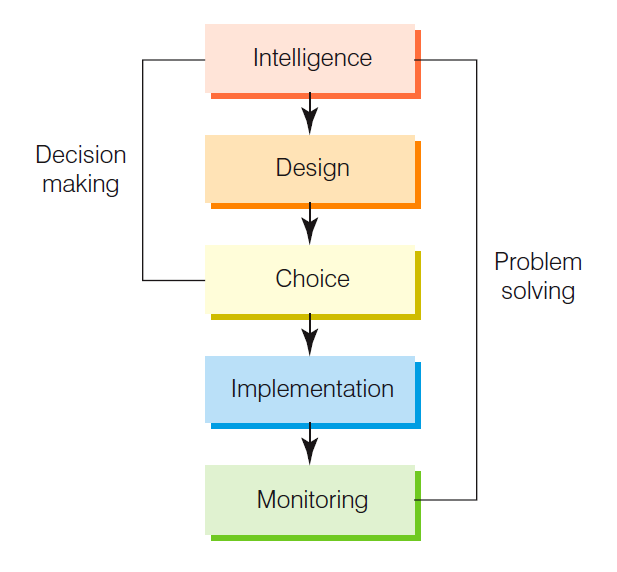
\includegraphics[width=0.9\linewidth]{chapter08/decision_making.png}
				\end{minipage}
				\begin{minipage}{0.6\textwidth}
					\begin{description}[]
						\item[Intelligence Stage] The first stage of decision-making, in which problems or opportunities are identified and defined.
						\item[Design Stage] The second stage of decision-making, in which alternative solutions to the problem are defined.
						\item[Choice Stage] The third stage of decision-making, which requires selecting a course of action.
						\item[Implementation Stage] A stage of problem-solving, in which a solution is put into effect.
						\item[Monitoring Stage] The final stage of the problem-solving process, in which decision-makers evaluate the implementation.
					\end{description}
				\end{minipage}
			\end{sidenote}
			\subsection{Programmed vs Non-Programmed Decisions}
				\begin{definition}{Programmed Decision}
					A decision made using a rule, procedure, or quantitative method.

					East to computerise using traditional information systems. They are structured, and deal with routine, well-defined decisions.
				\end{definition}
				\begin{definition}{Non-programmed Decision}
					A decision that deals with unusual or exceptional situations that can be difficult to quantify.
				\end{definition}
			\subsection{Optimisation, Satisficing, and Heuristic Approaches}
				\begin{definition}{Optimisation Model}
					A model that finds the best solution. These models use problem constraints.
				\end{definition}
				\begin{definition}{Satisficing Model}
					A model that will find a good, but not necessarily the best, problem solution.

					Usually used because modelling the problem properly to get an optimal decision would be too difficult, complex, or costly.

					Satisficing does not look at all possible solutions, but only those likely to give good results.
				\end{definition}
				\begin{definition}{Heuristics}
					Often referred to as \concept{rules of thumb}. Commonly accepted guidelines of procedures that usually find a good solution.
				\end{definition}
			\subsection{Sense and Respond}
				\begin{definition}{Sense and Respond (SaR)}
					Determining problems or opportunities (\concept{sense}), and developing systems to solve the problems or take advantage of the opportunities (\concept{respond}).

					Requires nimble organisations that replace traditional lines of authority with those that are flexible and dynamic.
				\end{definition}
			\subsection{Big Data}
				\begin{definition}{Big Data}
					Where the data that a company collects is so huge that it is difficult to process using traditional database technology.
				\end{definition}

		\pagebreak
		\section{An Overview of Management Information Systems}
			\begin{definition}{Management Information System (MIS)}
				An integrated collection of people, procedures, databases, hardware, and software, that provides managers and decision-makers with information to help achieve organisational goals.

				The primary purpose of an MIS is to help an organisation achieve its goals, by providing managers with insight into the regular operations of the organisation, so that they can control, organise, and plan more effectively.
			\end{definition}
			\subsection{Inputs to a Management Information System}
				Data enters an MIS from both internal and external sources.

				The most significant internal data sources are the organisation's various ERP and TPS systems.

				External sources of data can include customers, suppliers, competitors and stockholders, as well as other sources, such as the Internet.
			\subsection{Outputs of a Management Information System}
				The output is typically a collection of reports that are distributed to managers. These can include tabulations, summaries, charts, and graphs.
				\begin{definition}{Scheduled Reports}
					Reports that are produced periodically, or on a schedule, such as daily, weekly, or monthly.
				\end{definition}
				\begin{definition}{Key-Indicator Reports}
					Reports that summarise the previous day's critical activities. Typically, available at the beginning of each workday.

					Used to take quick, corrective action on significant aspects of the business.
				\end{definition}
				\begin{definition}{Demand Reports}
					Reports that are developed to give certain information at someone's request.
				\end{definition}
				\begin{definition}{Exception Reports}
					Reports that are automatically produced when a situation is unusual, or requires managerial action.
				\end{definition}
				\begin{definition}{Drill-down Reports}
					Reports that provide increasingly detailed data about a situation.

					Analyst can see data at a high level first, then at a more detailed level, then at a very detailed level.
				\end{definition}
				\begin{sidenote}{Developing Effective Reports}
					\begin{multicols}{2}
						\begin{itemize}[nosep]
							\item Tailor each report to user needs
							\item Spend time and effort producing only reports that are useful
							\item Pay attention to report content and layout
							\item Use management-by-exception reporting
							\item Set parameters carefully
							\item Produce all reports in a timely fashion
							\item Periodically review reports
						\end{itemize}
					\end{multicols}
				\end{sidenote}
			\subsection{Characteristics of a Management Information System}
				\begin{sidenote}{Functions of an MIS}
					\begin{multicols}{2}
						\begin{itemize}[nosep]
							\item Provide reports with fixed and standard formats
							\item Produce hard-copy and soft-copy reports
							\item Use internal data stored in the computer system
							\item Allow users to develop their own custom reports
							\item Require users to submit formal requests for reports to systems personnel
						\end{itemize}
					\end{multicols}
				\end{sidenote}

		\section{Functional Manufacturing Information Systems}
			\subsection{Financial Management Information Systems}
				\begin{definition}{Financial Management Information System}
					A management information system that provides financial information, not only for executives, but also for a broader set of people who need top make better decisions on a daily basis.
				\end{definition}
				\begin{sidenote}{Functions of a Financial MIS}
						\begin{itemize}[nosep]
							\item Integrate financial and operational information from multiple sources, including the Internet, into a single system.
							\item Provide easy access to data for both financial and non-financial users, often through the use of a corporate intranet.
							\item Make financial data immediately available to shorten analysis turnaround time
							\item Enable analysis of financial data along multiple dimensions
							\item Analyse historical and current financial activity
							\item Monitor and control the use of funds over time
						\end{itemize}
					Used to compute revenues, costs, profits, \concept{auditing}, as well as to manage funds.
					\begin{definition}{Auditing}
						Analysing the financial condition of an organisation, and determining whether financial statements and reports produced by the financial MIS are accurate.
					\end{definition}
				\end{sidenote}
			\subsection{Manufacturing Management Information Systems}
				\begin{definition}{Manufacturing Information System}
					A management information system that allows greater control over the manufacturing process.

					The manufacturing MIS subsystems and outputs monitor and control the flow of materials, products, and services throughout the organisation.
				\end{definition}
				\begin{sidenote}{Common Information Subsystems and Outputs in Manufacturing}
					\begin{description}
						\item[Design and engineering] Manufacturing companies often use \concept{computer-aided design (CAD)} with new or existing products.
						\item[Master production scheduling and inventory control] Provide detailed plans for both short-term and long-range scheduling of manufacturing facilities.
							\begin{description}[nosep]
								\item[Economic Order Quantity (EOQ)] The quantity that should be reordered to minimise total inventory costs.
								\item[Reorder Point (ROP)] A critical inventory quantity level.
								\item[Material Requirements Planning (MRP)] A set of inventory-controlled techniques that help coordinate thousands of inventory items when the demand for one item is dependent on the demand for another.
								\item[Just-in-time (JIT) Inventory] A philosophy of inventory management in which inventory and materials are delivered just before they are used in manufacturing a product.
							\end{description}
						\item[Process Control] Technologies used to control and streamline the manufacturing process.
							\begin{description}[nosep]
								\item[Computer-Aided Manufacturing (CAM)] A system that directly controls manufacturing equipment.
								\item[Computer-Integrated Manufacturing] Using computers to link the components of the production process into an effective system.
								\item[Flexible Manufacturing System (FMS)] An approach allowing manufacturing facilities to rapidly and efficiently change from making one product to making another.
							\end{description}
						\item[Quality Control] A process that ensures that the finished product meets the customer's needs.
					\end{description}
				\end{sidenote}
			\subsection{Marketing Management Information Systems}
				\begin{definition}{Marketing Management Information System}
					An information system that supports managerial activities in product development, distribution, pricing decisions, promotional effectiveness, and sales forecasting.
					\begin{description}
						\item[Customer Relationship Management (CRM)] Help a company manage all aspects of customer encounters. 
					\end{description}
				\end{definition}
				\pagebreak
				\begin{sidenote}{Subsystems of Marketing MIS}
					\begin{description}
						\item[Marketing Research] Conduct a formal study of the market and customer preferences.
						\item[Product Development] The conversion of raw materials into finished goods and services, focuses primarily on the physical attributes of the product.
						\item[Promotion and Advertising]
						\item[Product Pricing] Retail price, wholesale price, and price discounts must be set.
						\item[Sales Analysis] Identify products, sales personnel, and customers that contribute to profits, and those that do not.
							\begin{description}[nosep]
								\item[Sales-by-product report] Lists all major products and their sales for a period of time.
								\item[Sales-by-salesperson] Lists total sales for each salesperson. Can also be subdivided by product.
								\item[Sales-by-customer] Used to identify high- and low-volume customers.
							\end{description}
					\end{description}
				\end{sidenote}
			\subsection{Human Resource Management Information Systems}
				\begin{definition}{Human Resource Management Information System (HRMIS)}
					Also called a \concept{personnel MIS}. An information system that is concerned with activities related to employees and potential employees of an organisation.
				\end{definition}
				\begin{sidenote}{Subsystems of HRMIS}
					\begin{description}
						\item[Human Resource Planning] Put the right number and kinds of employees in the right jobs when they are needed.
						\item[Personnel Selection and Recruiting]
						\item[Training and Skills Inventory]
						\item[Scheduling and Job Placement]
						\item[Wage and Salary Administration]  
					\end{description}
				\end{sidenote}
			\subsection{Geographic Information Systems}
				\begin{definition}{Geographic Information System (GIS)}
					A computer system capable of assembling, storing, manipulating and displaying \concept{geographic information} (data that is identified according to its location).
					\begin{description}
						\item[Geographic Information] Data identified according to its location.
					\end{description}
				\end{definition}

	\vbox{\rulechapterend}
\end{document}